\section*{II.1.1}
Linear Discriminant Analysis with $m>2$ classes is done by creating a
discriminant function for each class and running each function on all points we
wish to classify. The discimination functions calculates the posterior
probability that a point belongs to its class, and so the one with the highest
probability is chosen.
The discrimination function for a class $k$ looks like
\[
  \delta_k(x) = x^\text{T}\Sigma^{-1}\mu_k - 
  \frac{1}{2}\mu^{\text{t}}_k\Sigma^{-1}\mu_k + \text{ln Pr}(Y = C_k)
\]
The prior distribution is calculated like
\[
  \text{Pr}(Y = C_k) = \ell_k / \ell
\]
Where $\ell$ is the number of elements in the training data, and $\ell_k$ is the
number of elements of class $k$ in the training data. $\mu_k$ is the mean of a
given class, while $\Sigma$ as the covariance matrix for each class added
together and normalized. They're calculated like so
\begin{align*}
  \mu_k  &= \frac{1}{\ell_k}\sum_{(x,y) \in S_k}x \\
  \Sigma &= \frac{1}{\ell - m}\sum_{k=1}^{m}\sum_{(x,y) \in S_k}(x-\mu_k)(x-\mu_k)^{\text{T}}
\end{align*}
Where $S_k$ is the points in the training set that corresponds to the class $k$
and $m$ is the number of classes.

Using this method we get an error of $14.00\%$ on the training data and
$21.05\%$ on the test data.

\section*{II.1.2}
The training error on the transformed data is $14\%$ and the test error on
the transformed data is $21.05\%$. This is exactly the same as it is on
the un-transformed data, as the standardization of the data makes no
difference for Linear Discriminant Analysis.

LDA discovers a number of functions which compute a posterior probability of the input,
which in rough terms is equivalent to calculating the probability that a given input comes
from that particular distribution (which is Gaussian in our case). In the end all that matters is
which of the functions produce the largest posterior probability, which is a
relative score compared to the other functions. Standardizing the data has no effect on this decision,
as the separating bounds between the probabilities remain the same relative to one another,
standardized data or no.

\section*{II.1.3}

The Bayes optimal classifier is given as the formula
\[
   c_{\text{BayesOpt}} = \underset{c_j \in C}{\text{argmax}} \sum_{h_i \in H}\text{P}(c_j|h_i)\text{P}(h_i|S)
\]
Where $H$ is every hypothesis given and $S$ is the training data.

In this assignment we're given two hypothesis ``The label 1 shows up in three fourths of all trials.''
along with the training data $S = \{(0,0), (0,1), (0,1), (0,1)\}$ which reflects the hypothesis.

In our case, $c_{\text{BayesOpt}}$ will always be that there is a bigger propability for the label being $1$ than $0$.

The Bayes optimal risk for this is $0.25$ or $25\%$. This is the minimum risk over all the measurable hypothesis in $H$, the hypothesis with the lowest risk is that the label should be $1$, which in our training set is true in $75\%$ of the cases and erronous in the remaining $25\%$.

Now we look at the probabilistic clasifier, that predicts 0 with a probability of $0.25$ and 1 with $0.75$.

Of the $0.25$ guesses on 0, $0.75$ will be wrong. Of the $0.75$ guesses on 1, $0.25$ will be wrong. So the sum of wrong answers is:

\begin{align*}
  0.25\cdot0.75 + 0.75\cdot0.25 &= 0.375
\end{align*}

So it would be better to always guess 1.

\pagebreak
\section*{II.2.1}
The RMS (Root Mean Square) error found on the test
set for each of the three selections was:

\begin{align*}
	RMS_1 = 35.4651 \\
	RMS_2 = 28.8398 \\
	RMS_3 = 18.7700
\end{align*}

Of the three models, selection 3 clearly provides
the best model, as can be seen both in Figure~\ref{fig:II_2_1_sel3} and by the RMS of
$18.7700$.

\FloatBarrier
\begin{figure}[h!]
	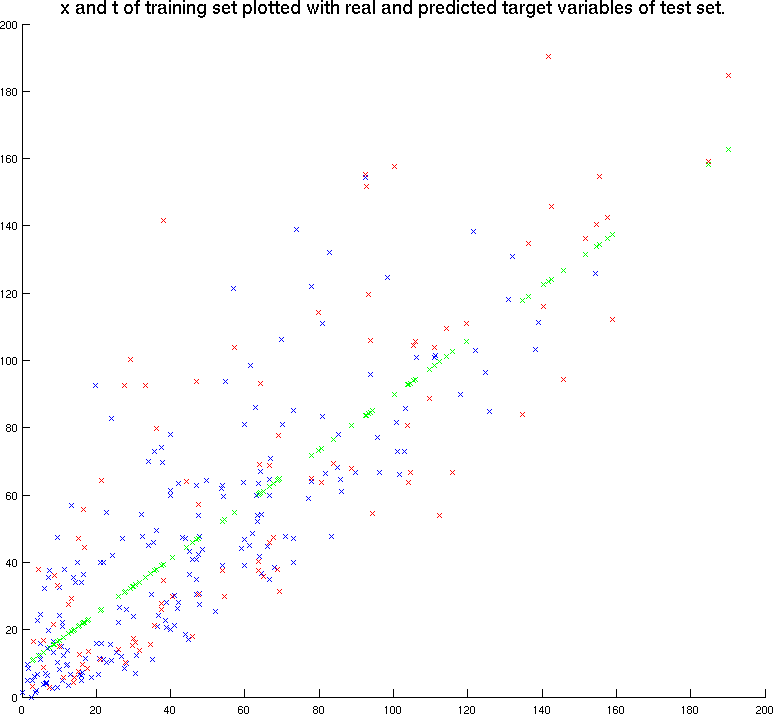
\includegraphics[width=\linewidth]{img/II_2_1_xt.png}
    \caption{\textit{x} and \textit{t} of training set, plotted 
    with real and predicted target variables.\label{fig:II_2_1_xt}}
\end{figure}

\begin{figure}[!ht]
	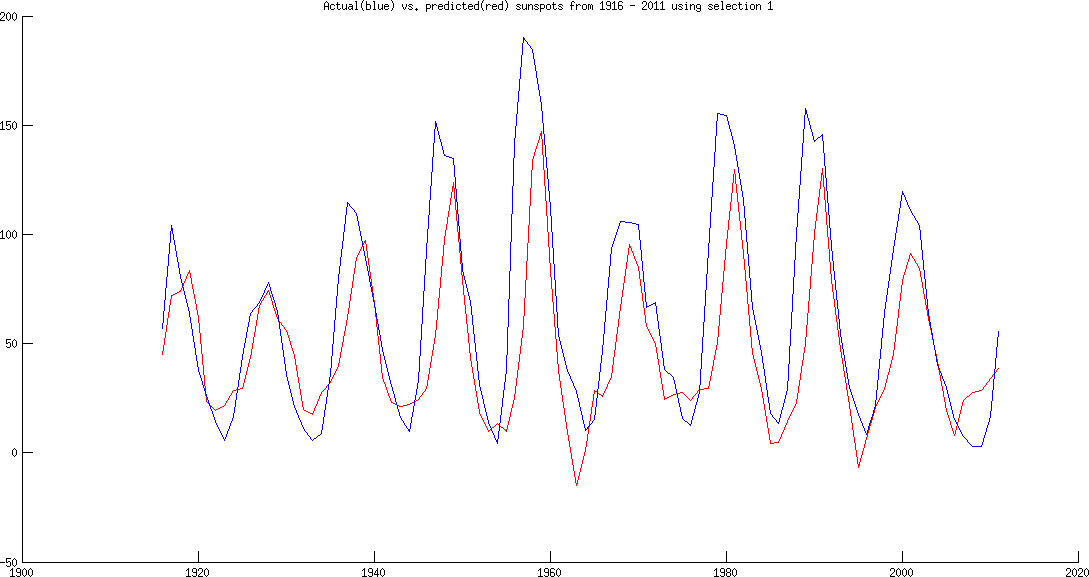
\includegraphics[width=\linewidth]{img/II_2_1_sel1.png}
    \caption{Years vs. predicted sunspot numbers, plotted with
    the true target values.\label{fig:II_2_1_sel1}}
\end{figure}

\begin{figure}[!ht]
	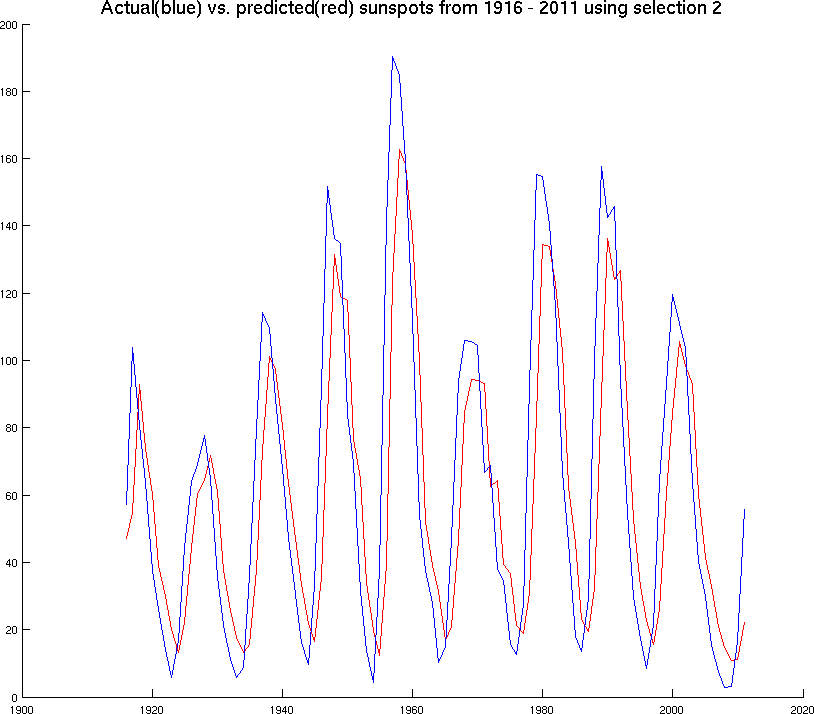
\includegraphics[width=\linewidth]{img/II_2_1_sel2.png}
    \caption{Years vs. predicted sunspot numbers, plotted with
    the true target values.\label{fig:II_2_1_sel2}}
\end{figure}

\begin{figure}[!ht]
	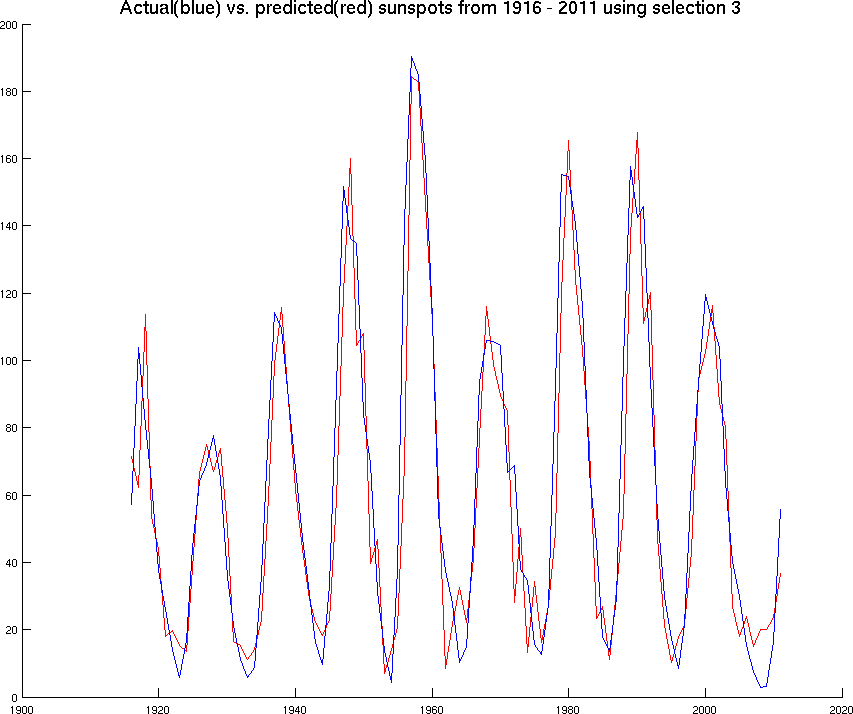
\includegraphics[width=\linewidth]{img/II_2_1_sel3.png}
    \caption{Years vs. predicted sunspot numbers, plotted with
    the true target values.\label{fig:II_2_1_sel3}}
\end{figure}

\FloatBarrier
\section*{II.2.2}
\begin{figure}[!ht]
	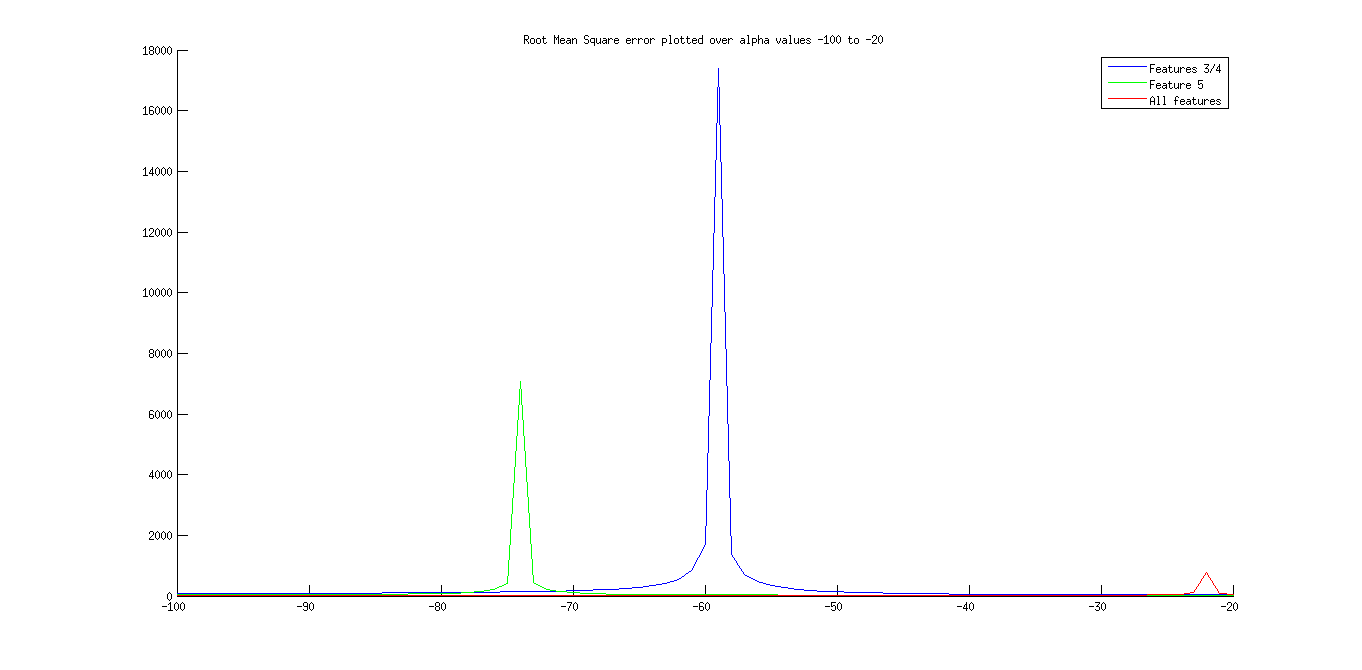
\includegraphics[width=\linewidth]{img/II_2_2_bad.png}
    \caption{RMS of each selection plotted against particularly badly chosen
    $\alpha$ values.\label{fig:II_2_2_bad}}
\end{figure}

\begin{figure}[!ht]
	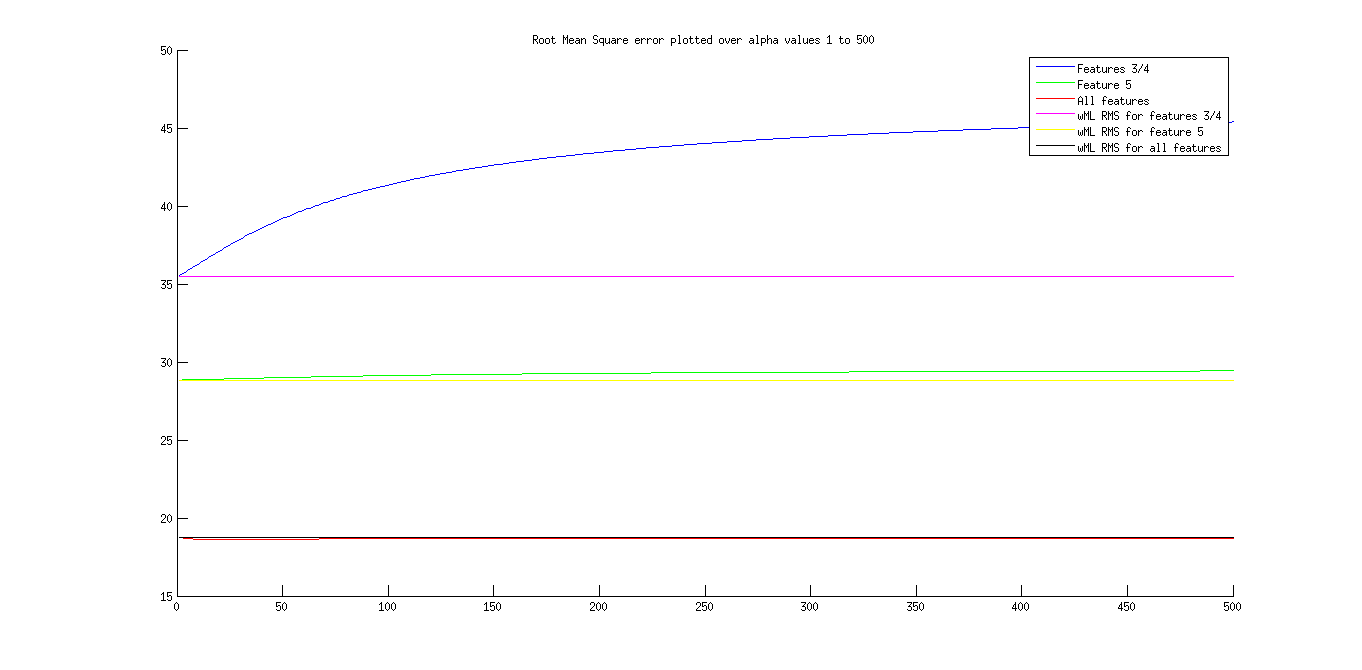
\includegraphics[width=\linewidth]{img/II_2_2_good.png}
    \caption{RMS of each selection and its corresponding $w_{ML}$-based model plotted against $\alpha$ values 1 to 500.\label{fig:II_2_2_good}}
\end{figure}

The model for selection 3 clearly performs best again, for most values of $\alpha$. We have been
unsure of what range of values to try with $\alpha$, and so we have tested all the way from -10000 to 10000.
There are some particularly bad $\alpha$-values in the negative range, at different points for the three different
selections. Figure~\ref{fig:II_2_2_bad} shows these peaks specifically, while Figure~\ref{fig:II_2_2_good} 
shows all 3 selections against the RMS obtained for that selection in \textsc{II.2.1}, for $\alpha$ values 1 to 500.
For selection 3, testing for $\alpha$-values between 0 and 10000, the RMS of selection 3 becomes lower for $\alpha$ values
0 to 7540.

In general, adjusting the alpha value seems to be a viable way to lower the prediction error; however, 
as Figure~\ref{fig:II_2_2_bad} shows, selecting bad $\alpha$ values can also result in disastrous prediction error.


\section*{II.2.3}

We look at:

\begin{align*}
  E_D(\textbf{w}) &= \frac{1}{2} \sum_{n=1}^{N} r_n
                     \{t_n-\textbf{w}^T
                     \phi(\textbf{x}_n)\}^2 \\
                  &= \frac{1}{2} \sum_{n=1}^{N} r_n
                     \left\{t_n-\sum_{m=1}^{|\textbf{w}|}w_m
                     \phi_m(\textbf{x}_n)\right\}^2
\end{align*}

To find $\textbf{w}^*$ that minimizes this
we find the partiel diffirentiated,
and set it equal $0$.
Here we diffirentiate with respect to
$w_i$, $0 < i < |\textbf{w}|$:

\begin{align*}
  (E_D(\textbf{w}))' &= \left(\frac{1}{2} \sum_{n=1}^{N} r_n
                        \left\{t_n-\sum_{m=1}^{|\textbf{w}|}
                        w_m \phi_m(\textbf{x}_n)
                        \right\}^2\right)'\\
                     &= \frac{1}{2} \sum_{n=1}^{N}
                        r_n \left(
                        \left\{t_n-\sum_{m=1}^{|\textbf{w}|}
                        w_m \phi_m
                        (\textbf{x}_n)\right\}^2\right)'
\end{align*}

Chain rule where:

\begin{align*}
  f(x)  &= x^2\\
  f'(x) &= 2x\\
  g(\textbf{w})  &= \left\{t_n-\sum_{m=1}^{|\textbf{w}|}
                    w_m \phi_m(\textbf{x}_n)\right\}\\
  g'(\textbf{w}) &= \left\{t_n-\sum_{m=1}^{|\textbf{w}|}
                    w_m \phi_m(\textbf{x}_n)\right\}'\\
                 &= -\phi_i(\textbf{x}_n)
\end{align*}

So:

\begin{align*}
  (E_D(\textbf{w}))' &= \frac{1}{2} \sum_{n=1}^{N}
                        r_n \left(2 \left\{
                        t_n-\sum_{m=1}^{|\textbf{w}|}
                        w_m \phi_m(\textbf{x}_n)
                        \right\} \cdot
                        -\phi_i(\textbf{x}_n)\right)\\
                     &= \sum_{n=1}^{N} r_n \left(
                        \left\{t_n-\sum_{m=1}^{|\textbf{w}|}
                        w_m \phi_m(\textbf{x}_n)
                        \right\} \cdot
                        -\phi_i(\textbf{x}_n)\right)\\
                     &= \sum_{n=1}^{N}
                        \left\{-r_n t_n\phi_i(\textbf{x}_n)
                        + \sum_{m=1}^{|\textbf{w}|}
                        r_n w_m \phi_m
                        (\textbf{x}_n)\phi_i
                        (\textbf{x}_n)\right\}
\end{align*}

Setting equal to $0$:

\begin{align*}
  (E_D(\textbf{w}))'           &= 0\\
  \sum_{n=1}^{N} \left\{-r_n t_n\phi_i(\textbf{x}_n)
  + \sum_{m=1}^{|\textbf{w}|} r_n w_m \phi_m(\textbf{x}_n)
  \phi_i(\textbf{x}_n)\right\} &= 0\\
  \sum_{n=1}^{N} \sum_{m=1}^{|\textbf{w}|} r_n w_m
  \phi_m(\textbf{x}_n)
  \phi_i(\textbf{x}_n) &= \sum_{n=1}^{N} r_n
  t_n\phi_i(\textbf{x}_n)\\
  \sum_{n=1}^{N} r_n \textbf{w}^T \phi(\textbf{x}_n)
  \phi_i(\textbf{x}_n) &= \sum_{n=1}^{N} r_n
  t_n\phi_i(\textbf{x}_n)
\end{align*}

As this count for every $0 < i < |\textbf{w}|$,
we can sum over every $i$:

\begin{align*}
  \sum_{i=1}^{|\textbf{w}|}
  \sum_{n=1}^{N} r_n \textbf{w}^T \phi(\textbf{x}_n)
  \phi_i(\textbf{x}_n) &= \sum_{i=1}^{|\textbf{w}|}
  \sum_{n=1}^{N} r_n t_n\phi_i(\textbf{x}_n) \\
  \sum_{n=1}^{N} r_n \textbf{w}^T \phi(\textbf{x}_n)
  \sum_{i=1}^{|\textbf{w}|}\phi_i(\textbf{x}_n) &=
  \sum_{n=1}^{N} r_n t_n
  \sum_{i=1}^{|\textbf{w}|}\phi_i(\textbf{x}_n)\\
  \sum_{n=1}^{N} r_n \textbf{w}^T \phi(\textbf{x}_n)
  \textbf{1}^T\phi(\textbf{x}_n) &=
  \sum_{n=1}^{N} r_n t_n
  \textbf{1}^T\phi(\textbf{x}_n)
\end{align*}

Which is something of the form:

\begin{align*}
  w_1\cdot C_1 + w_2\cdot C_2 + \ldots +
  w_{|\textbf{w}|}\cdot C_{|\textbf{w}|} &= K
\end{align*}

which yields a family of vectors $\textbf{w}$
minimizing the error function.

Intuition about weighted sum-of-squares:

\begin{description}
	\item[(i)] Data dependent noise variance: If we have domain knowledge
    then we can encode the domain knowledge into our error function
    by assuming some data-dependent level of noise for each individual
    sample.
    \item[(ii)] Replicated data points: If the data contains replicated
    data points, these risk becoming overly important for regular
    sum-of-squares. With weighted sum-of-squares we can proportionally
    reduce the importance of replicated points.
\end{description}